\chapter{Research Methodology and Analysis}
\label{ch:method}

This chapter describes how the research was carried out and presents its results. The first half
covers the methodology: the overall design (\cref{sec:method-design}), the data and the construction
of labels (\cref{sec:method-labels}), the structured model and its training (\cref{sec:method-rfdetr})
and the evaluation protocol (\cref{sec:method-eval}). The second half reports the results in the order
of the research questions (\cref{sec:res-labels} to \cref{sec:res-cost}).

\section{Research design}
\label{sec:method-design}

The study is a quantitative, experimental one. The benchmark of Zou et al.\ is rebuilt from public
annotations, since neither its labels nor its code are released, and every quantity that the paper does
not specify is treated as a free design choice, made on the basis of standard practice or of tuning on
held-out training data, and documented. Three principles guided all experiments:
\begin{enumerate}
  \item \textbf{No model selection on evaluation data.} Hyperparameters, score thresholds and the
        number of epochs are chosen on a \emph{tune split} of 10\% of the training scenes. Where the
        evaluation split is the official validation set (OpenLane-V2), the reported model is the last
        completed epoch, not the best one.
  \item \textbf{Controlled comparisons.} Comparisons change one factor at a time (the training data, the
        evaluation domain), with everything else, including the random seed, fixed.
  \item \textbf{Verifiable components.} Label builders are unit-tested and checked by hand on frames
        with difficult configurations; the metrics are unit-tested; the structured model is checked
        with a ground-truth oracle.
\end{enumerate}

All experiments ran on a single NVIDIA RTX~5070 (12\,GB) with PyTorch~2.14.1~\webcite{web:pytorch}, CUDA~13.0 and
the \code{rfdetr} library~1.11.2~\webcite{web:rfdetr}. The code is organized as a Python package (\code{dtsu}) with tools for data export,
training, evaluation and visualization; \cref{app:repro} lists the commands that reproduce every
number in this chapter.

\section{Data and label construction}
\label{sec:method-labels}

\subsection{OpenLane-V2}

Both subsets of OpenLane-V2~\webcite{web:openlanev2} are used, front camera only: \code{ring_front_center} of Argoverse~2 for
subset A (1550$\times$2048, portrait) and \code{CAM_FRONT} of nuScenes for subset B
(1600$\times$900). Since only the front-camera images are needed, only those were extracted from the
image archives, which bundle all cameras. The official validation split serves as evaluation set, as in
the original paper; the official test split has no usable annotations.

\paragraph{Rules.} Per-frame, per-maneuver labels are built from four annotations: the lane-to-traffic
element links (\code{topology_lcte}), the lane-to-lane links (\code{topology_lclc}), the centerline
geometry, and the traffic-element attribute (1 red, 2 green, 3 yellow, 4--12 arrow types). The procedure
has four steps (full details in \cref{app:labels}):
\begin{enumerate}
  \item \textbf{Maneuver per lane.} Each lane is followed along its successors to the first junction
        lane being entered, which must start no more than 3\,m behind the ego vehicle. The heading change
        along that junction lane gives the maneuver: within $30^\circ$ straight, beyond $135^\circ$
        U-turn, otherwise left or right by sign. U-turn is kept at this step only so that a light
        controlling nothing but U-turn lanes is not mistaken for a left-turn light; it is not an output.
  \item \textbf{Relevant lights.} Lights linked to lanes that are aligned with the ego heading (within
        $60^\circ$) and belong to the nearest junction (within 10\,m) are kept. If the ego vehicle has
        already passed the stop line, approach lanes ending within 30\,m behind it are used instead.
  \item \textbf{Lights to maneuvers.} The specificity hierarchy of \cref{sec:prob-semantics} assigns
        colors to maneuvers. The most specific light wins; when equally specific lights disagree, the
        frame is marked as a conflict.
  \item \textbf{Frame filter.} A frame is kept if at least one relevant colored light exists and there
        is no conflict (596 frames were dropped as conflicts).
\end{enumerate}

\paragraph{Validation.} Thirty validation frames covering five difficult cases (turn arrows,
straight~$=$~none, dedicated right signals, crossing the junction, conflicts) were inspected by eye.
The check revealed one error, a vehicle standing exactly at the stop line being assigned to the next
junction, which the 3\,m tolerance of step~1 corrects; all other inspected labels were correct or
plausible. \Cref{fig:examples} shows two labeled frames, and \cref{sec:res-labels} compares the
resulting distribution with the original paper.

\begin{table}[t]
\centering
\caption{Kept frames per split after label construction (OpenLane-V2, front camera).}
\label{tab:kept-frames}
\begin{tabular}{@{}lrr@{}}
\toprule
 & train & val \\
\midrule
Subset A & 10,141 / 22,477 & 2,220 / 4,806 \\
Subset B & 6,806 / 27,968 & 1,565 / 6,019 \\
A+B (this work) & 16,947 & 3,785 \\
Zou et al.~\cite{zou2026oneperception} & 23,904 & 5,147 \\
\bottomrule
\end{tabular}
\end{table}

\paragraph{Data scope.} The paper describes its benchmark as Subset-A, yet its frame counts (23,904
train, 5,147 val) exceed the total number of subset A frames \emph{before} any filtering (22,477 and
4,806). The paper's benchmark therefore cannot be subset A alone. Combining A and B fits its counts
better, and, as shown in \cref{sec:res-labels}, also its label distribution. All OpenLane-V2 models are
therefore trained on A+B and evaluated on subset A validation (the paper's reference set), subset B
validation and their union. \Cref{tab:kept-frames} lists the kept frames: this work keeps about 71\% as
many frames as the paper. The remaining difference cannot be resolved, since the paper's filtering
rules are not specified and it also applied manual quality control.

\paragraph{Tune split.} 10\% of the training scenes (70 per subset; 1,185 kept frames of A and 785 of
B) are held out as tune split. All hyperparameter decisions on OpenLane-V2 are made on it.

\subsection{DTLD and LISA}

Two further label builders produce records in the same format, so that datasets can be mixed and models
evaluated across them.

\paragraph{DTLD.} DTLD's \emph{relevant} flag marks lamps serving the route actually driven, which is
itself not annotated. The lamps serving each possible route are therefore re-derived from the
front-facing vehicle lamps at the ego intersection: a route with its own arrow is served by that arrow,
a route without one by the circles. Red--yellow (``prepare to go'') counts as red, since it still means
stop. Right turns follow the German rule (right arrow if present, otherwise the circle), recorded as
\code{near_turn = "signal"}; under this rule the training labels for right are 63\% green, 27\% red, 3\%
yellow and 7\% none, against 97\% none under the US convention. Frames are dropped for conflicting
lamps (619 in train), lamps that are off or of unknown state (656), disagreement with a reviewed
route-label rule (484), or the absence of a relevant vehicle lamp (949).

\paragraph{LISA.} LISA provides no relevance information. Lights at the ego intersection are identified
by size: a light is kept if it is at least 0.6 times as tall as the tallest light \emph{of the same
kind} (circle, left arrow, straight arrow). Comparing within a kind keeps far-side circles that would
otherwise be discarded next to a large near-side left-arrow pole, a case found during spot-checking.
Frames are dropped for conflicts (130 in train) and when only arrows are visible, because LISA leaves
some visible circles unannotated. Right is always \emph{none} under the US rule, since LISA has no
dedicated right-turn lights.

About 50 frames across both datasets were spot-checked on the same difficult cases as for OpenLane-V2.
Splits are listed in \cref{tab:ext-splits}: the official test sets are used for testing and a
validation split is held out from the official training data by whole sessions or clips.

\begin{table}[t]
\centering
\caption{Kept frames of the additional datasets. Images are resized to the canvas shown.}
\label{tab:ext-splits}
\begin{tabular}{@{}lrrrl@{}}
\toprule
 & train (fit) & val (tune) & test & canvas \\
\midrule
DTLD & 23,222 & 2,706 & 11,347 & 1024$\times$512 \\
LISA & 16,240 & 1,431 & 17,612 & 1024$\times$768 \\
\bottomrule
\end{tabular}
\end{table}

\section{The structured model}
\label{sec:method-rfdetr}

The model follows the structured paradigm of \cref{sec:prob-paradigms}: a detector classifies every
light by its color and by the ego maneuvers it controls, and an explicit rule turns the detections into
per-maneuver decisions.

\paragraph{Class encoding.} Every annotated light becomes one detection class \code{<moves>|<color>},
where \code{<moves>} is the set of ego maneuvers the light controls according to the label builder
(e.g.\ \code{left+straight}, \code{generic} for a circular light of the approach) or \code{irrelevant}
for lights of other lanes or junctions. On OpenLane-V2 A+B this gives 46 classes; on DTLD, whose
pictograms map to fewer combinations, 24.

\paragraph{Assignment rule.} At inference, detections above a score threshold are de-duplicated with
class-agnostic NMS (IoU 0.5) and their \code{<moves>} sets are passed to the same specificity hierarchy
used for the labels, with the highest score breaking ties between equally specific lights. The rule
takes the traffic convention as a parameter (US \emph{dedicated} or German \emph{signal} right turns).
Feeding ground-truth boxes through this rule reproduces every training label exactly (oracle TSS
$=1.0000$ on OpenLane-V2 and on DTLD fit, tune and test), so the model's errors are entirely due to
detection, classification and relevance.

\paragraph{Detector and training.} RF-DETR Medium (34.6M parameters) is fine-tuned from its released
detection-pretrained weights with the library's own recipe~\webcite{web:rfdetr} (optimizer, EMA, losses, schedule) except where it would corrupt
the labels: horizontal flips and random crops are disabled (a crop can remove the light that sets a
direction's label), multi-scale training is disabled in favor of a single square resolution of 1024
pixels, and brightness and contrast jitter is added (hue shifts are excluded because they change light
colors). The batch size is 4 with 4 gradient-accumulation steps. The complete settings are collected in
\cref{app:hparams} (\cref{tab:hparams-rfdetr}).

\paragraph{Tuning.} All model selection in this thesis (hyperparameters, epochs, score thresholds) was
done with four-direction scores, before U-turn was dropped; the selections are kept as they were made,
and the tune scores quoted for them are four-direction scores. On the tune split, RF-DETR Medium with
the default learning rate (tune TSS 0.905)
was better than Medium with half the learning rate (0.893) and than Large (0.896), and its tune TSS
plateaued after two epochs with a best score threshold of 0.20. The final model was trained for four
epochs on the full A+B training set with this threshold fixed, and the last epoch is reported; its
per-epoch results are listed in \cref{app:epochs} (\cref{tab:rfdetr-epochs}).

\paragraph{DTLD model.} The same recipe was trained on DTLD's fit split for 15 epochs, with a per-epoch
overfitting report: the eval-mode detection loss and the direction metrics on the held-out tune split
are compared with those on a fixed 1,000-frame probe of the training data. The tune split picks both
the epoch and the score threshold; DTLD test is only reported.

\section{Evaluation protocol}
\label{sec:method-eval}

All six metrics of \cref{sec:prob-metrics} are computed by one unit-tested function. Per-direction
results report $\acccolor$, $\accpass$, False-Go, False-Stop, the number of stop labels and the majority
baseline.

\paragraph{Statistical comparison.} Frames of the same driving segment are strongly correlated, so a
frame-level test would overstate the evidence. Two models are compared with a \emph{paired,
segment-level bootstrap}~\cite{efron1993introduction}: whole segments are resampled with replacement
(separately for the 112 segments of subset A val and the 65 of subset B val), both models are scored on
the same resample, and 10,000 resamples give a 95\% percentile interval and a two-sided p-value for the
difference of each metric.

\paragraph{Out-of-distribution evaluation.} A model trained on one dataset is scored on another only
after a label oracle check: every ground-truth light of the target is mapped to the model's class names
and pushed through the assignment rule with the target's traffic convention, and frames whose labels
cannot be reproduced this way are left out and counted (none of LISA; 1 of 2,220 frames of subset A
val). Any remaining gap is thus due to the detector. Results are given at two thresholds---the one
picked on the source tune split (the honest out-of-distribution number) and the best one on the
target's tune split (to measure how much of the gap is miscalibration)---and with two geometries:
squeezing the image to the square input, or first padding it to the 2:1 aspect ratio of the training
images.

% ---------------------------------------------------------------------------------------------------
\section{Results: label reconstruction}
\label{sec:res-labels}

\Cref{fig:label-dist} and \cref{tab:label-dist} compare the per-direction color distribution of the
reconstructed labels (A+B, train and val, kept frames) with Fig.~3 of the original paper.

\begin{figure}[t]
\centering
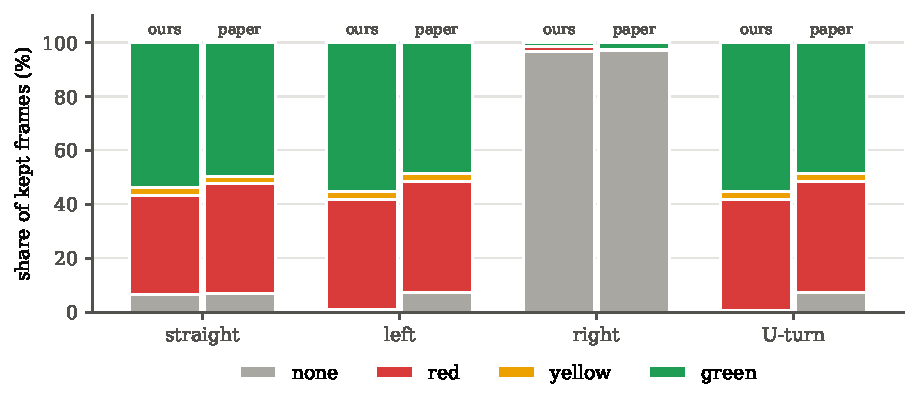
\includegraphics[width=\textwidth]{label_distribution.pdf}
\caption{Per-direction color distribution of the reconstructed labels (left bar of each pair) and of the
original benchmark (right bar, from Fig.~3 of Zou et al.).}
\label{fig:label-dist}
\end{figure}

\begin{table}[t]
\centering
\caption{Label distribution in \%, this work / Zou et al.\ (A+B, train + val, kept frames).}
\label{tab:label-dist}
\begin{tabular}{@{}lcccc@{}}
\toprule
Direction & none & red & green & yellow \\
\midrule
straight & 6.5 / 7.0 & 36.9 / 40.7 & 53.9 / 49.7 & 2.7 / 2.5 \\
left & 0.9 / 7.2 & 40.8 / 41.3 & 55.5 / 48.8 & 2.9 / 2.8 \\
right & 96.6 / 96.9 & 1.8 / 0.3 & 1.5 / 2.7 & 0.1 / 0.2 \\
\bottomrule
\end{tabular}
\end{table}

The distributions agree closely for straight and right, and for the colored classes of left. The
paper's Fig.~3 also shows U-turn, with a distribution nearly identical to left's; in the labels rebuilt
here U-turn takes the left signal in 99.9\% of the frames, which is why it is not used as a maneuver in
this thesis (\cref{sec:prob-def}). Two
observations support the reading that the original benchmark is A+B under US rules: subset A alone is
much greener (straight 28\% red, 64\% green), and mirroring the rules for the left-hand traffic scenes
of Singapore gives right~$=$~none in only 85.7\% of frames, far from the paper's 96.9\%. The one clear
mismatch is \emph{none} for left (0.9\% here, 7.2\% in the paper): in the paper, left
\emph{none} is about as frequent as straight \emph{none}, which suggests that its left labels inherit a
straight \emph{none} more often than the rules adopted here do.

\begin{figure}[t]
\centering
\begin{subfigure}[b]{0.36\textwidth}
  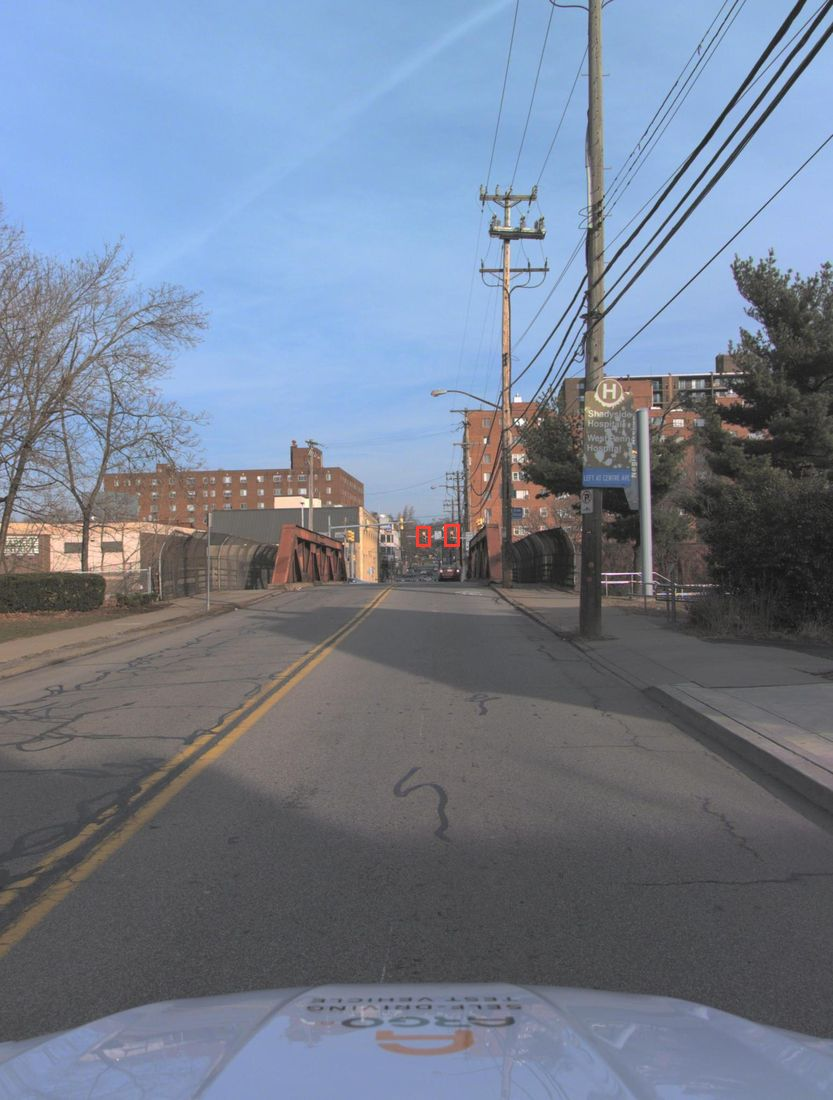
\includegraphics[width=\textwidth]{example_A-0004.jpg}
  \caption{Subset A (Argoverse 2)}
\end{subfigure}\hfill
\begin{subfigure}[b]{0.6\textwidth}
  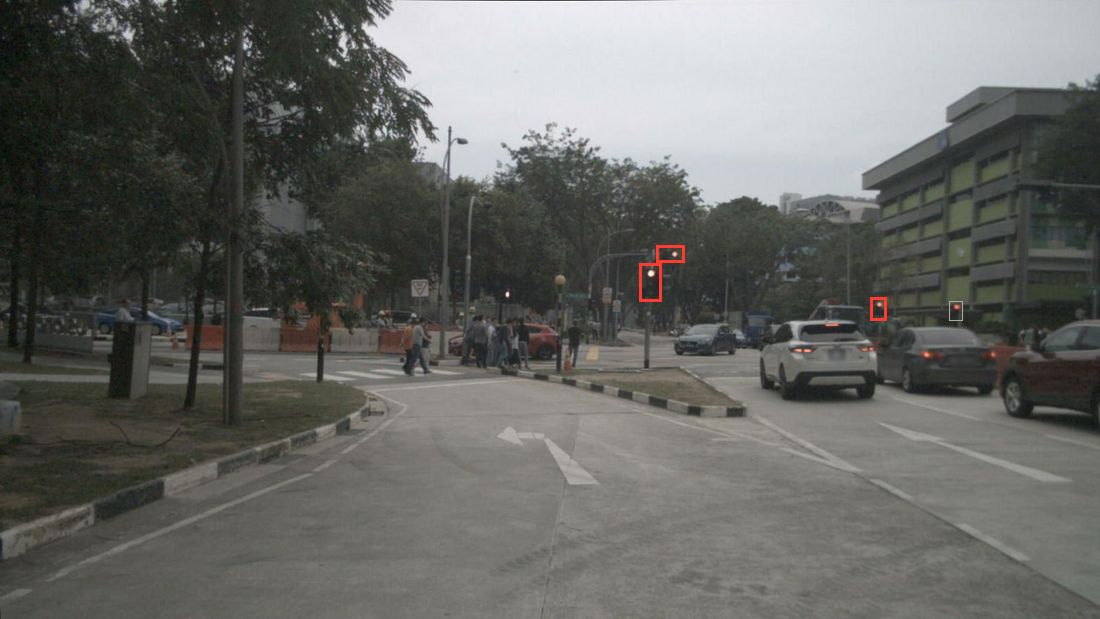
\includegraphics[width=\textwidth]{example_B-0028.jpg}
  \caption{Subset B (nuScenes, Singapore)}
\end{subfigure}
\caption{Validation frames with their annotated lights: lights the label builder marks as relevant for
the ego vehicle are outlined in their signal color, all other lights with a thin grey box.}
\label{fig:examples}
\end{figure}

\section{Results: structured model on OpenLane-V2}
\label{sec:res-openlane}

\begin{table}[t]
\centering
\caption{The structured model (RF-DETR-M, epoch 3, threshold 0.20) on OpenLane-V2 validation, over three
directions. The published values of Zou et al.\ are given for orientation only: they are over four
directions (U-turn included) and on the original, unreleased labels.}
\label{tab:openlane}
\small\setlength{\tabcolsep}{4pt}
\begin{tabular}{@{}lcccccc@{}}
\toprule
 & $\acccolor\uparrow$ & $\accpass\uparrow$ & $\EM\uparrow$ & $\TSS\uparrow$ & $\FG\downarrow$ & $\FS\downarrow$ \\
\midrule
Subset A val & 0.9147 & 0.9474 & 0.8351 & 0.8991 & 0.1516 & 0.0267 \\
Subset B val & 0.9306 & 0.9585 & 0.8569 & 0.9153 & 0.1118 & 0.0134 \\
A+B val & 0.9213 & 0.9520 & 0.8441 & 0.9058 & 0.1319 & 0.0215 \\
\midrule
\emph{Zou et al., direction-aware model} & \emph{0.9019} & \emph{0.9356} & \emph{0.8031} & \emph{0.8802} & \emph{0.1372} & \emph{0.0416} \\
\bottomrule
\end{tabular}
\end{table}

\Cref{tab:openlane} gives the overall result. On subset A val the structured model reaches a TSS of
0.899, and 0.915 on subset B, which is easier on every metric. The numbers lie in the range that Zou et
al.\ report for their direction-aware model (0.880 on their Subset-A), but the two are not directly
comparable: the labels are reconstructed, the number of kept frames differs (\cref{tab:kept-frames}),
and the paper's values include the U-turn. The per-epoch results (\cref{tab:rfdetr-epochs}) vary by about
one TSS point.

\paragraph{Per direction.} The original paper reports no per-direction results. \Cref{tab:perdir-A} and
\cref{fig:perdir} break the subset A results down by maneuver.

\begin{table}[t]
\centering
\caption{Per-direction results of the structured model on subset A val (2,220 frames). GT mix lists
none/red/yellow/green in \%. ``Maj.'' is the color accuracy of always predicting the most frequent color.}
\label{tab:perdir-A}
\small\setlength{\tabcolsep}{3pt}
\begin{tabular}{@{}lccccrc@{}}
\toprule
Direction & GT mix (\%) & $\acccolor$ & $\accpass$ & $\FG$ & \#stop & Maj. \\
\midrule
straight & 3.9 / 28.6 / 5.0 / 62.5 & 0.873 & 0.929 & 0.129 & 636 & 0.625 \\
left & 0.9 / 32.8 / 4.1 / 62.2 & 0.892 & 0.921 & 0.162 & 729 & 0.622 \\
right & 97.7 / 0.6 / 0.1 / 1.5 & 0.979 & 0.992 & 0.643 & 14 & 0.977 \\
\bottomrule
\end{tabular}
\end{table}

\begin{figure}[t]
\centering
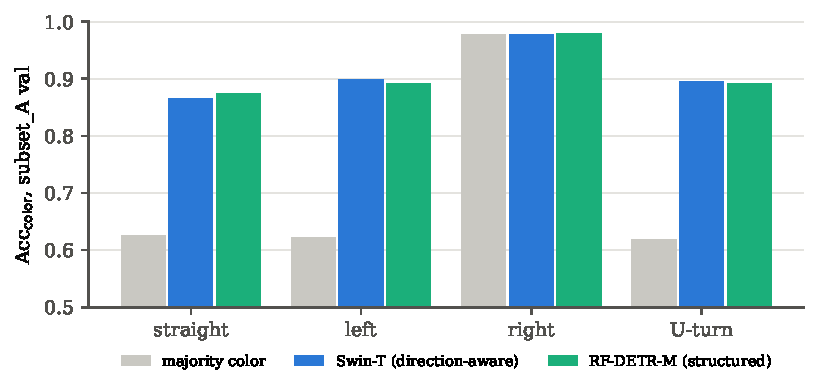
\includegraphics[width=0.85\textwidth]{per_direction.pdf}
\caption{Color accuracy per direction on subset A val, compared with the majority-color baseline.}
\label{fig:perdir}
\end{figure}

\paragraph{Straight and left are learned well.} Their color accuracy is well above the majority
baseline (25 and 27 points on subset A). Straight is the harder of the two on subset A (0.873). Its
\emph{none} class---no light governs straight, as at T-junctions or in turn-only lanes---is rarely
recognized: recall 0.17 on A (87 frames) and 0.46 on B (48 frames).

\paragraph{The right turn is not learned.} Its color accuracy equals the majority baseline (A: 0.979 vs
0.977; B: 0.950 vs 0.958): the model predicts \emph{none} almost always. The few red right-turn signals
(14 frames in A val, 37 in B val) are mostly missed, giving a right-turn False-Go of 0.64 on A and 0.84
on B. These cases are too few to affect the pooled False-Go, yet they are exactly the situations in
which a right turn is forbidden. Zou et al.'s label distribution has the same imbalance (right
\emph{none} 96.9\%), so this is a property of the data rather than of the model.

\paragraph{Yellow is weak on subset A.} Straight yellow recall is 0.53 on A (110 frames) against 0.68 on
B (34 frames); yellow is mostly confused with red or green. Since A has more yellow examples than B, this
is not only a sample-size effect; the amber rendering of Argoverse~2's camera, which makes yellow lamps
resemble red ones, is a likely contributor.

\paragraph{Passability follows color.} In the structured pipeline the passability is derived from the
color by the rule, so the two are consistent by construction, and all go/stop errors stem from color
errors, mainly red confused with green or yellow.

\section{Results: training and testing on DTLD}
\label{sec:res-dtld}

\begin{figure}[t]
\centering
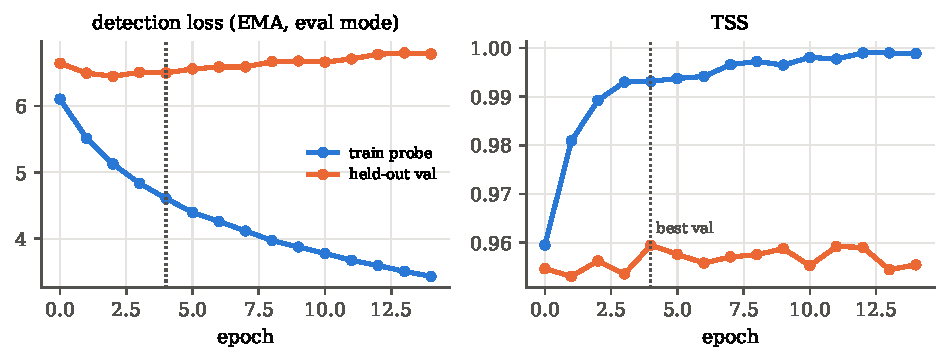
\includegraphics[width=\textwidth]{dtld_overfitting.pdf}
\caption{Overfitting report of the RF-DETR model trained on DTLD: detection loss and TSS on a fixed
probe of the training data and on the held-out tune split. The dotted line marks the best tune epoch.
TSS over four directions, as computed during training for the epoch selection.}
\label{fig:dtld-overfit}
\end{figure}

Trained on DTLD's fit split, the structured model reaches its best tune TSS of 0.9595 (four directions)
at epoch~4
(\cref{fig:dtld-overfit}). Afterwards the model overfits: the probe loss keeps falling (from 4.61 at
epoch 4 to 3.43 at epoch 14) and the probe TSS approaches 1.0, while the tune loss rises (6.50 to 6.79)
and the tune TSS stops improving. About five epochs are therefore sufficient.

\begin{table}[t]
\centering
\caption{RF-DETR-M on DTLD test (11,347 frames, German right-turn rule).}
\label{tab:dtld}
\small
\begin{tabular}{@{}lcccccc@{}}
\toprule
 & $\acccolor$ & $\accpass$ & $\EM$ & $\TSS$ & $\FG$ & $\FS$ \\
\midrule
Epoch 4 (best tune), thr.\ 0.25 & 0.966 & 0.979 & 0.928 & 0.958 & 0.034 & 0.015 \\
Epoch 14 (last), thr.\ 0.30 & 0.966 & 0.978 & 0.928 & 0.958 & 0.032 & 0.017 \\
\midrule
\multicolumn{7}{@{}l}{\emph{Per direction, epoch 14 ($\acccolor$ / $\accpass$ / $\FG$ / majority)}} \\
straight & \multicolumn{6}{l}{0.974 / 0.983 / 0.030 / 0.654} \\
left & \multicolumn{6}{l}{0.975 / 0.980 / 0.021 / 0.571} \\
right & \multicolumn{6}{l}{0.948 / 0.973 / 0.050 / 0.617} \\
\bottomrule
\end{tabular}
\end{table}

On DTLD test (\cref{tab:dtld}) the model reaches a TSS of 0.958 with a False-Go rate of only 0.034, far
lower than on OpenLane-V2. Under German rules right is no longer trivial (majority accuracy 0.617, with
3,231 stop labels), and it is the weakest direction (color accuracy 0.948), but it is clearly learned:
its False-Go rate is 0.050, against 0.64--0.89 for the rare right-turn reds of OpenLane-V2. Overfitting
after epoch 4 costs nothing on test: the last epoch gives the same TSS. Inference takes 22\,ms per frame
on the RTX~5070 (bf16, batch 1), or 37\,ms including JPEG decoding and resizing.

Why DTLD is so much easier than OpenLane-V2 cannot be settled with the experiments at hand. Plausible
contributors are that its relevance is derived from the route actually driven rather than from a lane
graph, that the training set is larger and drawn from a single camera setup, and that its 2:1 images lose
less resolution when resized to the square input than the portrait Argoverse~2 images do. The labels are
also built by different rules, so the two scores measure related but not identical tasks.

\section{Results: out-of-distribution evaluation}
\label{sec:res-ood}

The DTLD model (epoch 4, threshold 0.25) was evaluated without any retraining on LISA test and on
OpenLane-V2 validation, both under the US right-turn rule. \Cref{tab:ood} summarizes the results.

\begin{table}[t]
\centering
\caption{Out-of-distribution results of the DTLD-trained RF-DETR model (source threshold 0.25, images
squeezed to the square input). ``no right'' excludes the right direction. In-domain references: DTLD test
TSS 0.958; RF-DETR trained on OpenLane-V2: A 0.899, B 0.915.}
\label{tab:ood}
\small\setlength{\tabcolsep}{4pt}
\begin{tabular}{@{}lrcccccc@{}}
\toprule
Target & frames & $\TSS$ & $\TSS$ no right & $\acccolor$ & $\EM$ & $\FG$ & $\FS$ \\
\midrule
LISA test & 17,612 & 0.916 & 0.900 & 0.892$^\ast$ & 0.863 & 0.041$^\ast$ & 0.078$^\ast$ \\
\quad day & 7,306 & -- & 0.952 & & & & \\
\quad night & 10,306 & -- & 0.863 & & & & \\
OpenLane-V2 A val & 2,219 & 0.875 & 0.850 & 0.889 & 0.813 & 0.331 & 0.010 \\
OpenLane-V2 B val & 1,565 & 0.887 & 0.885 & 0.908 & 0.824 & 0.177 & 0.031 \\
\bottomrule
\multicolumn{8}{@{}l}{\footnotesize $^\ast$ without the right direction (always \emph{none} on LISA).}
\end{tabular}
\end{table}

\paragraph{LISA.} By day the model transfers well: a no-right TSS of 0.952 is close to its in-domain
DTLD performance, despite a different country and camera. At night the TSS drops to 0.863. Unlike on
OpenLane-V2, errors lean towards False-Stop (0.078) rather than False-Go (0.041). Since a missed light
leaves a maneuver at \emph{none}, which means \emph{go}, False-Stop errors come from lights read as red
that are not; at night, tail lights and other red light sources are plausible confusers. Neither
re-tuning the threshold on LISA's own tune split (no-right TSS 0.868) nor padding the images to the 2:1
training aspect (0.865) closes the gap, so it is not a calibration or geometry issue.

\paragraph{OpenLane-V2.} On nuScenes images (subset B) the DTLD model reaches a TSS of 0.887, three points
below the model trained in-domain (0.915). On Argoverse~2 images (subset A) the TSS drop is similar
(0.875 vs 0.899), but the False-Go rate more than doubles (0.331 vs 0.152): the model frequently declares
straight (False-Go 0.29) and left (0.35) maneuvers free when their signal is red. In the structured
pipeline a relevant light that is not detected leaves its maneuver at \emph{none}, that is, \emph{go}, so
missed red lights turn directly into False-Go errors. Two effects plausibly combine to cause the misses: the amber, red-leaning color rendering of the Argoverse~2 camera that already made yellow
hard in-domain, and the portrait geometry, which after squeezing into a square makes lights appear at a
different aspect ratio than in the wide DTLD images. Padding the portrait images to 2:1 instead makes
the lights even smaller and the results much worse (TSS 0.804, False-Go 0.48); threshold re-tuning
changes the results by less than half a point.

\section{Results: per-light evaluation on ATLAS}
\label{sec:res-atlas}

ATLAS has no relevance or maneuver labels, so the DTLD model is evaluated per light: each annotated light
is matched to the detections (class-agnostic, greedy by score, IoU $\ge$ 0.5), and detection recall and
precision, color accuracy on matched lights and, for arrows, whether the predicted maneuver set equals
the arrow's direction are measured. The evaluation uses the official ATLAS test
split of each camera; lights that are off are not among the model's classes and are not counted.

\begin{table}[t]
\centering
\caption{Per-light results of the DTLD-trained model on the three ATLAS cameras (IoU 0.5; in brackets
IoU 0.3).}
\label{tab:atlas}
\small
\begin{tabular}{@{}lrrcccc@{}}
\toprule
Camera & images & lights & recall & precision & color acc. & arrow moves acc. \\
\midrule
wide & 828 & 2,055 & 0.469 (0.585) & 0.569 (0.723) & 0.962 & 0.436 \\
medium & 1,003 & 2,064 & 0.658 (0.729) & 0.644 (0.731) & 0.887 & 0.468 \\
tele & 997 & 2,050 & 0.679 (0.759) & 0.606 (0.698) & 0.895 & 0.481 \\
\bottomrule
\end{tabular}
\end{table}

\begin{figure}[t]
\centering
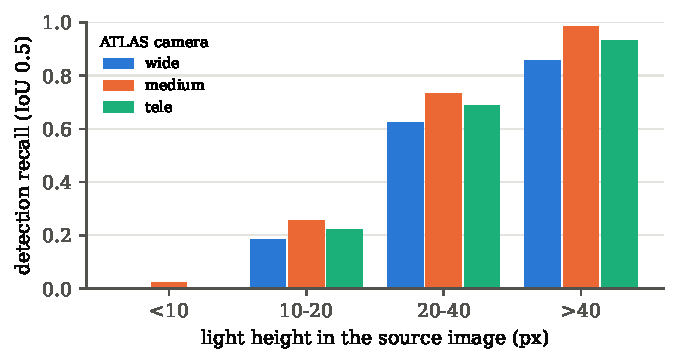
\includegraphics[width=0.75\textwidth]{atlas_recall.pdf}
\caption{Detection recall on ATLAS as a function of the light's height in the source image.}
\label{fig:atlas}
\end{figure}

\Cref{tab:atlas} and \cref{fig:atlas} show that detection is the bottleneck. Recall depends almost
entirely on the light's size: lights taller than 40 pixels are found in 86--98\% of the cases, lights of
20--40 pixels in 62--73\%, lights of 10--20 pixels in only about 20\%, and lights below 10 pixels
practically never. The wide camera, whose lights are smallest, has the lowest recall. The much higher
recall at IoU 0.3 indicates that a part of the misses are localization errors on small boxes rather than
missed lights. Color, once a light is detected, is recognized with 89--96\% accuracy. The arrow result is
the weakest: for fewer than half of the matched arrows does the predicted maneuver set equal the arrow's
direction. Part of this is by design: the model's classes encode the maneuvers a light controls for the ego
vehicle, as derived from the DTLD route labels, not the pictogram as such, so an arrow can legitimately
receive a broader class such as the one used for circles. Even so, the result shows that the model does
not reliably carry over pictogram recognition to a new camera setup.

\section{Computational cost}
\label{sec:res-cost}

\Cref{tab:cost} collects the cost of the models trained in this work.

\begin{table}[t]
\centering
\caption{Model size and training cost on one RTX 5070.}
\label{tab:cost}
\small
\begin{tabular}{@{}lrrll@{}}
\toprule
Model & Params & Epochs & Time / epoch & Peak mem. \\
\midrule
RF-DETR-M, OpenLane-V2 & 34.6M & 4 & $\approx$20 min & 6.5 GiB \\
RF-DETR-M, DTLD & 34.6M & 15 & $\approx$27 min & 6.6 GiB \\
\bottomrule
\multicolumn{5}{@{}l}{\footnotesize Time per epoch including validation.} \\
\end{tabular}
\end{table}

A few epochs of fine-tuning suffice on both datasets, and at inference the model runs at 22\,ms per
frame (\cref{sec:res-dtld}), comfortably within the frame rate of automotive cameras.
